\documentclass{jsarticle}
\usepackage[dvipdfmx]{graphicx}
\usepackage{amsmath,amssymb}
\newtheorem{dfn}{定義}
\newtheorem{thm}{定理}
\newtheorem{pps}{命題}

\pagestyle{myheadings}

\begin{document}

\title{「The “echo state” approach to analysing and training recurrent neural networks」のまとめ}
\author{市村 剛大}
\maketitle

\section*{概要}
echo state networkとは出力層のみ学習するリカレントニューラルネットワークである

\section{Echo states}

\begin{figure}[htbp]
  \centering
  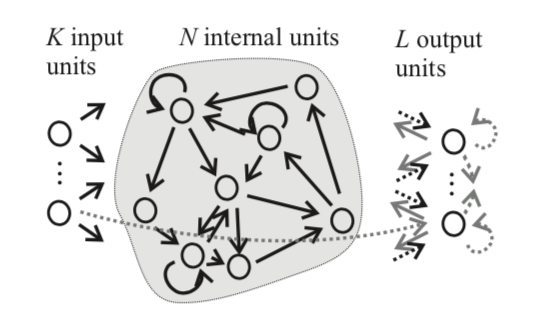
\includegraphics[width=0.5\hsize]{./figures/esn.png}
  \caption{echo state networkの基本構成}
  \label{fig:basic_structure}
\end{figure}

図\ref{fig:basic_structure}のようなニューラルネットワークを考える。
入力数$K$、ニューロン数$N$、出力数$L$であり、ある時間$n$での入力ベクトルを${\bf u}(n) = (u_1(n),...,u_K(n))$、内部状態ベクトルを${\bf x}(n) = (x_1(n),...,x_N(n))$、出力ベクトルを${\bf y}(n) = (y_1(n),...,y_L(n))$とする。また$N\times K$の入力層荷重行列を${\bf W}^{in}$、$N\times N$の内部結合荷重行列を$\bf W$、$L\times (K+L+N)$の出力層行列を${\bf W}^{out}$、そして$N\times L$の出力層から内部ニューロンへの戻り値行列を${\bf W}^{back}$とする。このとき、内部状態は次式のように更新される。
\begin{equation}
	{\bf x}(n+1)={\bf f}({\bf W}^{in}{\bf u}(n+1)+{\bf W}{\bf x}(n)+{\bf W}^{back}{\bf y}(n)),
	\label{eq:increment_x}
\end{equation}
ここで$\bf f$は活性化関数(ベクトル)である。また出力ベクトル${\bf y}(n+1)$は次式のように得られる。
\begin{equation}
	{\bf y}(n+1)={\bf f}^{out}({\bf W}^{out}({\bf u}(n+1),{\bf x}(n+1),{\bf y}(n))),
	\label{eq:increment_y}
\end{equation}
${\bf f}^{out}$は出力層の活性化関数(ベクトル)である。以降簡単のために入力${\bf u}(n)$のシークエンス(入力列)を表\ref{tb:u_shorthand}のように略記する。
\begin{table}[htb]
\caption{入力${\bf u}(n)$のシークエンス(列)の略記法}
\centering
  \begin{tabular}{cl}
    ${\bf \bar u}^{\pm \infty}$ & 左右無限大の入力列\\
    ${\bf \bar u}^{+ \infty}$ & 右に無限大に続く入力列\\
    ${\bf \bar u}^{- \infty}$ & 左に無限大に続く入力列\\
    ${\bf \bar u}^{k}$ & 長さ$k$の入力列
  \end{tabular}
  \label{tb:u_shorthand}
\end{table}
また、演算子$T$を導入し、入力列${\bf \bar u}^{k}$が入力されたのちの内部状態を${\bf x}(x+h) = T({\bf x}(n),{\bf y}(n),{\bf \bar u}^{k})$のように表すこととする。これは、出力層からのフィードバックがない場合は${\bf x}(x+h) = T({\bf x}(n),{\bf \bar u}^{k})$となる。
このとき、以下のように出力からのフィードバックがない場合のecho state networkを定義する。
\begin{dfn}
標準コンパクト性条件\footnote{(i)入力がコンパクト集合$U$から得ること、(ii)ネットワーク状態がコンパクトセット$A$に属すこと。}が成立し、ネットワークが出力層からのフィードバックを持たない場合を考える。このとき、もしネットワークの状態${\bf x}(n)$が左に無限の入力列${\bf \bar u}^{- \infty}$によって一意に決まるならば、ネットワークはecho stateを持つ。さらに正確にいえば、すべての入力ベクトル、ネットワークの状態に対して、${\bf x}(i) = T({\bf x}(i-1),{\bf u}(i))$と${\bf x'}(i) = T({\bf x'}(i-1),{\bf u}(i))$が存在するならば、${\bf x}(n)={\bf x'}(n)$である。
\end{dfn}
echo state propertyは次のように記述することもできる。入力echo関数${\bf E}=(e_{1},...,e_{N})$が存在し、$e_{i}:U^{-\mathbb{N}} \rightarrow \mathbb{R}$のとき、すべての左に無限の入力列履歴に対して、現在の状態は
\begin{equation}
	{\bf x}(n)={\bf E}(...,{\bf u}(n-1),{\bf u}(n))
\end{equation}
のように表せる。
\begin{dfn}
(a)$\forall i< n$に対して$T({\bf x}(i),{\bf u}(i+1))={\bf x}(i+1)$とき、左に無限の状態列${\bf \bar x}^{- \infty}$は左に無限の入力列${\bf \bar u}^{- \infty}$と互換性がある(compatible)と呼ぶ。
(b)同様に、$\forall i$に対して$T({\bf x}(i),{\bf u}(i+1))={\bf x}(i+1)$とき、左右に無限の状態列${\bf \bar x}^{\infty}$は左右に無限の入力列${\bf \bar u}^{\infty}$と互換性がある。
(c)もし状態列$...,{\bf x}(n-1),{\bf x}(n)$が存在するならば、$T({\bf x}(i),{\bf u}(i+1))={\bf x}(i+1)$かつ${\bf x}={\bf x}(n)$であるとき、ネットワーク状態${\bf x}\in A$は入力列${\bf \bar u}^{- \infty}$と終端互換性がある(end-compatible)と呼ぶ。
(d)もし${\bf x}(n-h),...,{\bf x}(n) \in A^{h+1}$が存在するならば、$T({\bf x}(i),{\bf u}(i+1))={\bf x}(i+1)$かつ${\bf x}={\bf x}(n)$であるとき、ネットワーク状態${\bf x} \in A$は入力列${\bf \bar u}^{h}$と終端互換性がある(end-compatible)と呼ぶ。
\end{dfn}
\begin{dfn}
標準コンパクト条件が成立し、出力層からのフィードバックがないとする。
\begin{enumerate}
\item すべての右側に無限な入力列${\bf \bar u}^{+ \infty}$に対して、null列$(\delta_{h})_{{h}\geq 0}$が存在する場合を考える。すべての状態${\bf x},{\bf x'} \in A$、すべての$h \geq 0$、すべての有限入力列${\bf \bar u}^{h}={\bf u}(n),...,{\bf u}(n+h)$について$d(T({\bf x},{\bf \bar u}^{h}),T({\bf x'},{\bf \bar u}^{h}))<\delta_{h}$となるとき、これを状態契約(state contracting)であるという。ここで$d$は$\mathbb{R}^{N}$上のユークリッド距離である。

\item すべての左側に無限な入力列${\bf \bar u}^{- \infty}$に対して、null列$(\delta_{h})_{{h}\geq 0}$が存在する場合を考える。すべての状態${\bf x},{\bf x'} \in A$、すべての$h \geq 0$、すべての有限入力列${\bf \bar u}^{h}={\bf u}(n-h),...,{\bf u}(n)$について$d(T({\bf x},{\bf \bar u}^{h}),T({\bf x'},{\bf \bar u}^{h}))<\delta_{h}$となるとき、これを状態忘却(state forgetting)であるという。

\item すべての左側に無限な入力列${\bf \bar u}^{- \infty}$に対して、null列$(\delta_{h})_{{h}\geq 0}$が存在する場合を考える。すべての状態${\bf x},{\bf x'} \in A$、すべての$h \geq 0$、すべての有限入力列${\bf \bar u}^{h}={\bf u}(n-h),...,{\bf u}(n)$、すべての${\bf \bar w^{- \infty}}{\bf \bar u}^{h},{\bf \bar w^{- \infty}}{\bf \bar u}^{h}$形式の左に無限の入力列、すべての${\bf \bar w^{- \infty}}{\bf \bar u}^{h}$と終端互換性がある${\bf x}$と${\bf \bar v^{- \infty}}{\bf \bar u}^{h}$と終端互換性がある${\bf x'}$について$d({\bf x},{\bf x})<\delta_{h}$となるとき、これを入力忘却(input forgetting)であるという。
\end{enumerate}
\end{dfn}
\begin{pps}
標準コンパクト条件が成立し、出力層からのフィードバックがない場合を考える。$T$が状態、入力のなかで連続であると仮定する。このとき状態契約、状態忘却、入力忘却の特性は、すべてネットワークがecho statesを持っているということに等しい。
\end{pps}
\begin{pps}
標準コンパクト条件が成立し、出力層からのフィードバックがない場合を考える。$T$が状態、入力のなかで連続である、echo statesであるとする。このとき、すべての左に無限の入力列${\bf \bar u}^{- \infty}$について、すべての$\epsilon >0$に対して、$d({\bf u}(k),{{\bf u}'}(k))<\delta$(ただし$k$は$-h \geq k \geq 0$である任意の$k$)を満たすようなすべての入力列${\bf {\bar u}}'^{- \infty}$について$d({\bf E}({\bf \bar u}^{- \infty}),{\bf E}({\bf \bar u}'^{- \infty}))< \epsilon$となるような$\delta >0$と$h >0$が存在する。
\end{pps}
\begin{pps}
活性化関数ユニット$f_{i}=\tanh$である場合を考える。(a)荷重行列$W$が$\sigma_{max}=\Lambda < 1$を満たすとする。ここで$\sigma_{max}$は最大の特異値である。このとき、すべての状態${\bf x},{\bf x'}\in [-1,1]^{N}$について$d(T({\bf x},{\bf u}),T({\bf x'},{\bf u}))< \Lambda d({\bf x}, {\bf x'})$となる。(b)荷重行列がスペクトル半径$|\lambda_{max}|>1$であるとする。ここで$\lambda_{max}$は$W$の最大の固有値である。このときネットワークは漸近的不安定null状態(asymptotically unstable null state)を持つ。これは、このネットワークが任意の0を含む入力セット$U$、許容される状態セット$A=[-1,1]^{N}$に対して、echo statesを持たないということを意味する。
\end{pps}
\end{document}
\bye
%%%%%%%%%%%%%%%%%TRASHBOX%%%%%%%%%%%%%%%%%%%%%%%%%%%%%